\chapter{\label{results}Results}
 The ground state configuration of kagome lattice with anisotropic ferromagnetic interaction along z-axis and DMI as a rich phase diagram (Fig-1 in \cite{sen_seshadri}). Spin-wave band structure for bulk and strip geometry is present for the phase with ground state configuration having all spins pointing along \textit{z}-direction.
 
\begin{figure}[!h]
                \centering
                \begin{tikzpicture}[scale = 0.75]
                \foreach \x in {0,2,...,8}
				{\draw[thick, o-] (\x,0)--(\x+1,0);
				\draw[thick,-o] (\x,1.73)--(\x+1,1.73);
				\node[below,red] at (\x,1.73) {{\footnotesize A}};
				\node[below] at (\x+1,1.73) {{\footnotesize B}};
				\node[left,blue] at (\x+0.5,2.6) {{\footnotesize C}};
				\draw[thick, o-] (\x,3.46)--(\x+1,3.46);
				\node[below,red] at (\x+1,3.46) {{\footnotesize A}};
				\draw[thick, -] (\x,5.2)--(\x+1,5.2);};		
			\foreach \x in {1,3,5,7} 
				{\node[below,red] at (\x,0) {{\footnotesize A}};
				 \draw[thick,*-] (\x,0)--(\x+1,0);
				 \node[below] at (\x+1,0) {{\footnotesize B}};
				 \node[left,blue] at (\x+0.5,0.87) {{\footnotesize C}};
				 \draw[thick,-*] (\x,1.73)--(\x+1,1.73);
				 \draw[thick,*-] (\x,3.46)--(\x+1,3.46);
				 \node[below] at (\x+1,3.46) {{\footnotesize B}};
				 \node[left,blue] at (\x+0.5,4.33) {{\footnotesize C}};
				 \draw[thick,-] (\x,5.2)--(\x+1,5.2);};
			\foreach \x in {1,3,5}
				{\draw[thick] (\x,0) -- (\x+3.5,6.06);};
			\draw[thick] (7,0) -- (9,3.46);
			\draw[thick] (2,0) -- (0,3.46);
			\draw[thick] (0,1.73)--(2.5,6.06);
			\draw[thick] (9,1.73)--(6.5,6.06);
			\foreach \x in {4,6,8}
				{\draw[thick] (\x,0) -- (\x-3.5,6.06);
				\node[below,red] at (\x,5.2) {{\footnotesize A}};
				\node[below] at (\x+1,5.2) {{\footnotesize B}};
				\node[left,blue] at (\x+0.5,6.06) {{\footnotesize C}};};
                \end{tikzpicture}
                \caption{Kagome lattice}
\end{figure}
 \begin{figure}
 \centering
        \begin{tikzpicture}[scale=3.5,cap=round,>=latex]
	% Radius of regular polygons
	\newdimen\R
	\R=0.8cm
	\coordinate (center) at (0,0);
	\draw (0:\R)
	\foreach \x in {60,120,...,360} {  -- (\x:\R) }
%	-- cycle (300:\R) node[below] {$\csc \theta$}
%	-- cycle (240:\R) node[below] {$\sec \theta$}
%	-- cycle (180:\R) node[left] {$\tan \theta$}
%	-- cycle (120:\R) node[above] {$\sin \theta$}
%	-- cycle (60:\R) node[above] {$\cos \theta$}
	-- cycle (0:0) node[right] {$ \Gamma $}
	-- cycle (0:\R) node[right] {$ \mathrm{K} $}
	-- cycle (30:0.9*\R) node[right] {$\mathrm{M}$};
	\draw[->,thick] (0,0) -- cycle (30:0.9*\R);
	\end{tikzpicture}
        \caption{First Brillouin zone}
\end{figure}
% \begin{figure}[!h]
%     \centering
%     \resizebox{0.5\textwidth}{!}{% GNUPLOT: LaTeX picture
\setlength{\unitlength}{0.240900pt}
\ifx\plotpoint\undefined\newsavebox{\plotpoint}\fi
\sbox{\plotpoint}{\rule[-0.200pt]{0.400pt}{0.400pt}}%
\begin{picture}(1500,900)(0,0)
\sbox{\plotpoint}{\rule[-0.200pt]{0.400pt}{0.400pt}}%
\put(171.0,82.0){\rule[-0.200pt]{4.818pt}{0.400pt}}
\put(151,82){\makebox(0,0)[r]{-1}}
\put(1430.0,82.0){\rule[-0.200pt]{4.818pt}{0.400pt}}
\put(171.0,179.0){\rule[-0.200pt]{4.818pt}{0.400pt}}
\put(151,179){\makebox(0,0)[r]{ 0}}
\put(1430.0,179.0){\rule[-0.200pt]{4.818pt}{0.400pt}}
\put(171.0,277.0){\rule[-0.200pt]{4.818pt}{0.400pt}}
\put(151,277){\makebox(0,0)[r]{ 1}}
\put(1430.0,277.0){\rule[-0.200pt]{4.818pt}{0.400pt}}
\put(171.0,374.0){\rule[-0.200pt]{4.818pt}{0.400pt}}
\put(151,374){\makebox(0,0)[r]{ 2}}
\put(1430.0,374.0){\rule[-0.200pt]{4.818pt}{0.400pt}}
\put(171.0,471.0){\rule[-0.200pt]{4.818pt}{0.400pt}}
\put(151,471){\makebox(0,0)[r]{ 3}}
\put(1430.0,471.0){\rule[-0.200pt]{4.818pt}{0.400pt}}
\put(171.0,568.0){\rule[-0.200pt]{4.818pt}{0.400pt}}
\put(151,568){\makebox(0,0)[r]{ 4}}
\put(1430.0,568.0){\rule[-0.200pt]{4.818pt}{0.400pt}}
\put(171.0,666.0){\rule[-0.200pt]{4.818pt}{0.400pt}}
\put(151,666){\makebox(0,0)[r]{ 5}}
\put(1430.0,666.0){\rule[-0.200pt]{4.818pt}{0.400pt}}
\put(171.0,763.0){\rule[-0.200pt]{4.818pt}{0.400pt}}
\put(151,763){\makebox(0,0)[r]{ 6}}
\put(1430.0,763.0){\rule[-0.200pt]{4.818pt}{0.400pt}}
\put(171.0,860.0){\rule[-0.200pt]{4.818pt}{0.400pt}}
\put(151,860){\makebox(0,0)[r]{ 7}}
\put(1430.0,860.0){\rule[-0.200pt]{4.818pt}{0.400pt}}
\put(171.0,82.0){\rule[-0.200pt]{0.400pt}{4.818pt}}
\put(171,41){\makebox(0,0){$\Gamma$}}
\put(171.0,840.0){\rule[-0.200pt]{0.400pt}{4.818pt}}
\put(584.0,82.0){\rule[-0.200pt]{0.400pt}{4.818pt}}
\put(584,41){\makebox(0,0){$\mathrm{M}$}}
\put(584.0,840.0){\rule[-0.200pt]{0.400pt}{4.818pt}}
\put(1017.0,82.0){\rule[-0.200pt]{0.400pt}{4.818pt}}
\put(1017,41){\makebox(0,0){$\mathrm{K}$}}
\put(1017.0,840.0){\rule[-0.200pt]{0.400pt}{4.818pt}}
\put(1450.0,82.0){\rule[-0.200pt]{0.400pt}{4.818pt}}
\put(1450,41){\makebox(0,0){$\Gamma$}}
\put(1450.0,840.0){\rule[-0.200pt]{0.400pt}{4.818pt}}
\put(171.0,82.0){\rule[-0.200pt]{0.400pt}{187.420pt}}
\put(171.0,82.0){\rule[-0.200pt]{308.111pt}{0.400pt}}
\put(1450.0,82.0){\rule[-0.200pt]{0.400pt}{187.420pt}}
\put(171.0,860.0){\rule[-0.200pt]{308.111pt}{0.400pt}}
\put(70,471){\makebox(0,0){$\frac{E}{|JS|}$}}
\put(171,179){\usebox{\plotpoint}}
\put(171,178.67){\rule{5.059pt}{0.400pt}}
\multiput(171.00,178.17)(10.500,1.000){2}{\rule{2.529pt}{0.400pt}}
\put(192,180.17){\rule{4.100pt}{0.400pt}}
\multiput(192.00,179.17)(11.490,2.000){2}{\rule{2.050pt}{0.400pt}}
\multiput(212.00,182.60)(2.967,0.468){5}{\rule{2.200pt}{0.113pt}}
\multiput(212.00,181.17)(16.434,4.000){2}{\rule{1.100pt}{0.400pt}}
\multiput(233.00,186.59)(1.847,0.482){9}{\rule{1.500pt}{0.116pt}}
\multiput(233.00,185.17)(17.887,6.000){2}{\rule{0.750pt}{0.400pt}}
\multiput(254.00,192.59)(1.484,0.485){11}{\rule{1.243pt}{0.117pt}}
\multiput(254.00,191.17)(17.420,7.000){2}{\rule{0.621pt}{0.400pt}}
\multiput(274.00,199.59)(1.352,0.488){13}{\rule{1.150pt}{0.117pt}}
\multiput(274.00,198.17)(18.613,8.000){2}{\rule{0.575pt}{0.400pt}}
\multiput(295.00,207.58)(1.017,0.491){17}{\rule{0.900pt}{0.118pt}}
\multiput(295.00,206.17)(18.132,10.000){2}{\rule{0.450pt}{0.400pt}}
\multiput(315.00,217.58)(0.967,0.492){19}{\rule{0.864pt}{0.118pt}}
\multiput(315.00,216.17)(19.207,11.000){2}{\rule{0.432pt}{0.400pt}}
\multiput(336.00,228.58)(0.884,0.492){21}{\rule{0.800pt}{0.119pt}}
\multiput(336.00,227.17)(19.340,12.000){2}{\rule{0.400pt}{0.400pt}}
\multiput(357.00,240.58)(0.774,0.493){23}{\rule{0.715pt}{0.119pt}}
\multiput(357.00,239.17)(18.515,13.000){2}{\rule{0.358pt}{0.400pt}}
\multiput(377.00,253.58)(0.754,0.494){25}{\rule{0.700pt}{0.119pt}}
\multiput(377.00,252.17)(19.547,14.000){2}{\rule{0.350pt}{0.400pt}}
\multiput(398.00,267.58)(0.754,0.494){25}{\rule{0.700pt}{0.119pt}}
\multiput(398.00,266.17)(19.547,14.000){2}{\rule{0.350pt}{0.400pt}}
\multiput(419.00,281.58)(0.668,0.494){27}{\rule{0.633pt}{0.119pt}}
\multiput(419.00,280.17)(18.685,15.000){2}{\rule{0.317pt}{0.400pt}}
\multiput(439.00,296.58)(0.702,0.494){27}{\rule{0.660pt}{0.119pt}}
\multiput(439.00,295.17)(19.630,15.000){2}{\rule{0.330pt}{0.400pt}}
\multiput(460.00,311.58)(0.717,0.494){25}{\rule{0.671pt}{0.119pt}}
\multiput(460.00,310.17)(18.606,14.000){2}{\rule{0.336pt}{0.400pt}}
\multiput(480.00,325.58)(0.814,0.493){23}{\rule{0.746pt}{0.119pt}}
\multiput(480.00,324.17)(19.451,13.000){2}{\rule{0.373pt}{0.400pt}}
\multiput(501.00,338.58)(0.884,0.492){21}{\rule{0.800pt}{0.119pt}}
\multiput(501.00,337.17)(19.340,12.000){2}{\rule{0.400pt}{0.400pt}}
\multiput(522.00,350.58)(1.017,0.491){17}{\rule{0.900pt}{0.118pt}}
\multiput(522.00,349.17)(18.132,10.000){2}{\rule{0.450pt}{0.400pt}}
\multiput(542.00,360.59)(1.847,0.482){9}{\rule{1.500pt}{0.116pt}}
\multiput(542.00,359.17)(17.887,6.000){2}{\rule{0.750pt}{0.400pt}}
\put(563,366.17){\rule{4.300pt}{0.400pt}}
\multiput(563.00,365.17)(12.075,2.000){2}{\rule{2.150pt}{0.400pt}}
\put(625,367.67){\rule{4.818pt}{0.400pt}}
\multiput(625.00,367.17)(10.000,1.000){2}{\rule{2.409pt}{0.400pt}}
\put(645,368.67){\rule{5.059pt}{0.400pt}}
\multiput(645.00,368.17)(10.500,1.000){2}{\rule{2.529pt}{0.400pt}}
\put(666,369.67){\rule{5.059pt}{0.400pt}}
\multiput(666.00,369.17)(10.500,1.000){2}{\rule{2.529pt}{0.400pt}}
\multiput(687.00,371.61)(4.258,0.447){3}{\rule{2.767pt}{0.108pt}}
\multiput(687.00,370.17)(14.258,3.000){2}{\rule{1.383pt}{0.400pt}}
\put(707,374.17){\rule{4.300pt}{0.400pt}}
\multiput(707.00,373.17)(12.075,2.000){2}{\rule{2.150pt}{0.400pt}}
\multiput(728.00,376.61)(4.481,0.447){3}{\rule{2.900pt}{0.108pt}}
\multiput(728.00,375.17)(14.981,3.000){2}{\rule{1.450pt}{0.400pt}}
\multiput(749.00,379.61)(4.258,0.447){3}{\rule{2.767pt}{0.108pt}}
\multiput(749.00,378.17)(14.258,3.000){2}{\rule{1.383pt}{0.400pt}}
\multiput(769.00,382.60)(2.967,0.468){5}{\rule{2.200pt}{0.113pt}}
\multiput(769.00,381.17)(16.434,4.000){2}{\rule{1.100pt}{0.400pt}}
\multiput(790.00,386.60)(2.967,0.468){5}{\rule{2.200pt}{0.113pt}}
\multiput(790.00,385.17)(16.434,4.000){2}{\rule{1.100pt}{0.400pt}}
\multiput(811.00,390.60)(2.821,0.468){5}{\rule{2.100pt}{0.113pt}}
\multiput(811.00,389.17)(15.641,4.000){2}{\rule{1.050pt}{0.400pt}}
\multiput(831.00,394.59)(2.269,0.477){7}{\rule{1.780pt}{0.115pt}}
\multiput(831.00,393.17)(17.306,5.000){2}{\rule{0.890pt}{0.400pt}}
\multiput(852.00,399.60)(2.821,0.468){5}{\rule{2.100pt}{0.113pt}}
\multiput(852.00,398.17)(15.641,4.000){2}{\rule{1.050pt}{0.400pt}}
\multiput(872.00,403.59)(2.269,0.477){7}{\rule{1.780pt}{0.115pt}}
\multiput(872.00,402.17)(17.306,5.000){2}{\rule{0.890pt}{0.400pt}}
\multiput(893.00,408.59)(2.269,0.477){7}{\rule{1.780pt}{0.115pt}}
\multiput(893.00,407.17)(17.306,5.000){2}{\rule{0.890pt}{0.400pt}}
\multiput(914.00,413.59)(2.157,0.477){7}{\rule{1.700pt}{0.115pt}}
\multiput(914.00,412.17)(16.472,5.000){2}{\rule{0.850pt}{0.400pt}}
\multiput(934.00,418.60)(2.967,0.468){5}{\rule{2.200pt}{0.113pt}}
\multiput(934.00,417.17)(16.434,4.000){2}{\rule{1.100pt}{0.400pt}}
\multiput(955.00,422.61)(4.481,0.447){3}{\rule{2.900pt}{0.108pt}}
\multiput(955.00,421.17)(14.981,3.000){2}{\rule{1.450pt}{0.400pt}}
\multiput(976.00,425.61)(4.258,0.447){3}{\rule{2.767pt}{0.108pt}}
\multiput(976.00,424.17)(14.258,3.000){2}{\rule{1.383pt}{0.400pt}}
\put(996,427.67){\rule{5.059pt}{0.400pt}}
\multiput(996.00,427.17)(10.500,1.000){2}{\rule{2.529pt}{0.400pt}}
\put(584.0,368.0){\rule[-0.200pt]{9.877pt}{0.400pt}}
\multiput(1037.00,427.93)(2.269,-0.477){7}{\rule{1.780pt}{0.115pt}}
\multiput(1037.00,428.17)(17.306,-5.000){2}{\rule{0.890pt}{0.400pt}}
\multiput(1058.00,422.92)(1.069,-0.491){17}{\rule{0.940pt}{0.118pt}}
\multiput(1058.00,423.17)(19.049,-10.000){2}{\rule{0.470pt}{0.400pt}}
\multiput(1079.00,412.92)(0.668,-0.494){27}{\rule{0.633pt}{0.119pt}}
\multiput(1079.00,413.17)(18.685,-15.000){2}{\rule{0.317pt}{0.400pt}}
\multiput(1099.00,397.92)(0.657,-0.494){29}{\rule{0.625pt}{0.119pt}}
\multiput(1099.00,398.17)(19.703,-16.000){2}{\rule{0.313pt}{0.400pt}}
\multiput(1120.00,381.92)(0.583,-0.495){33}{\rule{0.567pt}{0.119pt}}
\multiput(1120.00,382.17)(19.824,-18.000){2}{\rule{0.283pt}{0.400pt}}
\multiput(1141.00,363.92)(0.554,-0.495){33}{\rule{0.544pt}{0.119pt}}
\multiput(1141.00,364.17)(18.870,-18.000){2}{\rule{0.272pt}{0.400pt}}
\multiput(1161.00,345.92)(0.551,-0.495){35}{\rule{0.542pt}{0.119pt}}
\multiput(1161.00,346.17)(19.875,-19.000){2}{\rule{0.271pt}{0.400pt}}
\multiput(1182.00,326.92)(0.525,-0.495){35}{\rule{0.521pt}{0.119pt}}
\multiput(1182.00,327.17)(18.919,-19.000){2}{\rule{0.261pt}{0.400pt}}
\multiput(1202.00,307.92)(0.583,-0.495){33}{\rule{0.567pt}{0.119pt}}
\multiput(1202.00,308.17)(19.824,-18.000){2}{\rule{0.283pt}{0.400pt}}
\multiput(1223.00,289.92)(0.618,-0.495){31}{\rule{0.594pt}{0.119pt}}
\multiput(1223.00,290.17)(19.767,-17.000){2}{\rule{0.297pt}{0.400pt}}
\multiput(1244.00,272.92)(0.588,-0.495){31}{\rule{0.571pt}{0.119pt}}
\multiput(1244.00,273.17)(18.816,-17.000){2}{\rule{0.285pt}{0.400pt}}
\multiput(1264.00,255.92)(0.702,-0.494){27}{\rule{0.660pt}{0.119pt}}
\multiput(1264.00,256.17)(19.630,-15.000){2}{\rule{0.330pt}{0.400pt}}
\multiput(1285.00,240.92)(0.754,-0.494){25}{\rule{0.700pt}{0.119pt}}
\multiput(1285.00,241.17)(19.547,-14.000){2}{\rule{0.350pt}{0.400pt}}
\multiput(1306.00,226.92)(0.841,-0.492){21}{\rule{0.767pt}{0.119pt}}
\multiput(1306.00,227.17)(18.409,-12.000){2}{\rule{0.383pt}{0.400pt}}
\multiput(1326.00,214.92)(0.967,-0.492){19}{\rule{0.864pt}{0.118pt}}
\multiput(1326.00,215.17)(19.207,-11.000){2}{\rule{0.432pt}{0.400pt}}
\multiput(1347.00,203.93)(1.135,-0.489){15}{\rule{0.989pt}{0.118pt}}
\multiput(1347.00,204.17)(17.948,-9.000){2}{\rule{0.494pt}{0.400pt}}
\multiput(1367.00,194.93)(1.560,-0.485){11}{\rule{1.300pt}{0.117pt}}
\multiput(1367.00,195.17)(18.302,-7.000){2}{\rule{0.650pt}{0.400pt}}
\multiput(1388.00,187.93)(1.847,-0.482){9}{\rule{1.500pt}{0.116pt}}
\multiput(1388.00,188.17)(17.887,-6.000){2}{\rule{0.750pt}{0.400pt}}
\multiput(1409.00,181.95)(4.258,-0.447){3}{\rule{2.767pt}{0.108pt}}
\multiput(1409.00,182.17)(14.258,-3.000){2}{\rule{1.383pt}{0.400pt}}
\put(1429,178.67){\rule{5.059pt}{0.400pt}}
\multiput(1429.00,179.17)(10.500,-1.000){2}{\rule{2.529pt}{0.400pt}}
\put(1017.0,429.0){\rule[-0.200pt]{4.818pt}{0.400pt}}
\put(171,679){\usebox{\plotpoint}}
\put(171,677.67){\rule{5.059pt}{0.400pt}}
\multiput(171.00,678.17)(10.500,-1.000){2}{\rule{2.529pt}{0.400pt}}
\put(212,676.17){\rule{4.300pt}{0.400pt}}
\multiput(212.00,677.17)(12.075,-2.000){2}{\rule{2.150pt}{0.400pt}}
\put(233,674.67){\rule{5.059pt}{0.400pt}}
\multiput(233.00,675.17)(10.500,-1.000){2}{\rule{2.529pt}{0.400pt}}
\multiput(254.00,673.95)(4.258,-0.447){3}{\rule{2.767pt}{0.108pt}}
\multiput(254.00,674.17)(14.258,-3.000){2}{\rule{1.383pt}{0.400pt}}
\multiput(274.00,670.95)(4.481,-0.447){3}{\rule{2.900pt}{0.108pt}}
\multiput(274.00,671.17)(14.981,-3.000){2}{\rule{1.450pt}{0.400pt}}
\multiput(295.00,667.95)(4.258,-0.447){3}{\rule{2.767pt}{0.108pt}}
\multiput(295.00,668.17)(14.258,-3.000){2}{\rule{1.383pt}{0.400pt}}
\multiput(315.00,664.93)(2.269,-0.477){7}{\rule{1.780pt}{0.115pt}}
\multiput(315.00,665.17)(17.306,-5.000){2}{\rule{0.890pt}{0.400pt}}
\multiput(336.00,659.93)(2.269,-0.477){7}{\rule{1.780pt}{0.115pt}}
\multiput(336.00,660.17)(17.306,-5.000){2}{\rule{0.890pt}{0.400pt}}
\multiput(357.00,654.93)(1.484,-0.485){11}{\rule{1.243pt}{0.117pt}}
\multiput(357.00,655.17)(17.420,-7.000){2}{\rule{0.621pt}{0.400pt}}
\multiput(377.00,647.93)(1.560,-0.485){11}{\rule{1.300pt}{0.117pt}}
\multiput(377.00,648.17)(18.302,-7.000){2}{\rule{0.650pt}{0.400pt}}
\multiput(398.00,640.93)(1.194,-0.489){15}{\rule{1.033pt}{0.118pt}}
\multiput(398.00,641.17)(18.855,-9.000){2}{\rule{0.517pt}{0.400pt}}
\multiput(419.00,631.92)(1.017,-0.491){17}{\rule{0.900pt}{0.118pt}}
\multiput(419.00,632.17)(18.132,-10.000){2}{\rule{0.450pt}{0.400pt}}
\multiput(439.00,621.92)(1.069,-0.491){17}{\rule{0.940pt}{0.118pt}}
\multiput(439.00,622.17)(19.049,-10.000){2}{\rule{0.470pt}{0.400pt}}
\multiput(460.00,611.92)(1.017,-0.491){17}{\rule{0.900pt}{0.118pt}}
\multiput(460.00,612.17)(18.132,-10.000){2}{\rule{0.450pt}{0.400pt}}
\multiput(480.00,601.92)(0.967,-0.492){19}{\rule{0.864pt}{0.118pt}}
\multiput(480.00,602.17)(19.207,-11.000){2}{\rule{0.432pt}{0.400pt}}
\multiput(501.00,590.93)(1.194,-0.489){15}{\rule{1.033pt}{0.118pt}}
\multiput(501.00,591.17)(18.855,-9.000){2}{\rule{0.517pt}{0.400pt}}
\multiput(522.00,581.93)(1.286,-0.488){13}{\rule{1.100pt}{0.117pt}}
\multiput(522.00,582.17)(17.717,-8.000){2}{\rule{0.550pt}{0.400pt}}
\multiput(542.00,573.93)(2.269,-0.477){7}{\rule{1.780pt}{0.115pt}}
\multiput(542.00,574.17)(17.306,-5.000){2}{\rule{0.890pt}{0.400pt}}
\put(563,568.17){\rule{4.300pt}{0.400pt}}
\multiput(563.00,569.17)(12.075,-2.000){2}{\rule{2.150pt}{0.400pt}}
\put(192.0,678.0){\rule[-0.200pt]{4.818pt}{0.400pt}}
\put(625,566.67){\rule{4.818pt}{0.400pt}}
\multiput(625.00,567.17)(10.000,-1.000){2}{\rule{2.409pt}{0.400pt}}
\put(645,565.67){\rule{5.059pt}{0.400pt}}
\multiput(645.00,566.17)(10.500,-1.000){2}{\rule{2.529pt}{0.400pt}}
\put(666,564.67){\rule{5.059pt}{0.400pt}}
\multiput(666.00,565.17)(10.500,-1.000){2}{\rule{2.529pt}{0.400pt}}
\put(687,563.17){\rule{4.100pt}{0.400pt}}
\multiput(687.00,564.17)(11.490,-2.000){2}{\rule{2.050pt}{0.400pt}}
\put(707,561.17){\rule{4.300pt}{0.400pt}}
\multiput(707.00,562.17)(12.075,-2.000){2}{\rule{2.150pt}{0.400pt}}
\put(728,559.17){\rule{4.300pt}{0.400pt}}
\multiput(728.00,560.17)(12.075,-2.000){2}{\rule{2.150pt}{0.400pt}}
\multiput(749.00,557.95)(4.258,-0.447){3}{\rule{2.767pt}{0.108pt}}
\multiput(749.00,558.17)(14.258,-3.000){2}{\rule{1.383pt}{0.400pt}}
\multiput(769.00,554.94)(2.967,-0.468){5}{\rule{2.200pt}{0.113pt}}
\multiput(769.00,555.17)(16.434,-4.000){2}{\rule{1.100pt}{0.400pt}}
\multiput(790.00,550.95)(4.481,-0.447){3}{\rule{2.900pt}{0.108pt}}
\multiput(790.00,551.17)(14.981,-3.000){2}{\rule{1.450pt}{0.400pt}}
\multiput(811.00,547.94)(2.821,-0.468){5}{\rule{2.100pt}{0.113pt}}
\multiput(811.00,548.17)(15.641,-4.000){2}{\rule{1.050pt}{0.400pt}}
\multiput(831.00,543.94)(2.967,-0.468){5}{\rule{2.200pt}{0.113pt}}
\multiput(831.00,544.17)(16.434,-4.000){2}{\rule{1.100pt}{0.400pt}}
\multiput(852.00,539.94)(2.821,-0.468){5}{\rule{2.100pt}{0.113pt}}
\multiput(852.00,540.17)(15.641,-4.000){2}{\rule{1.050pt}{0.400pt}}
\multiput(872.00,535.93)(2.269,-0.477){7}{\rule{1.780pt}{0.115pt}}
\multiput(872.00,536.17)(17.306,-5.000){2}{\rule{0.890pt}{0.400pt}}
\multiput(893.00,530.94)(2.967,-0.468){5}{\rule{2.200pt}{0.113pt}}
\multiput(893.00,531.17)(16.434,-4.000){2}{\rule{1.100pt}{0.400pt}}
\multiput(914.00,526.94)(2.821,-0.468){5}{\rule{2.100pt}{0.113pt}}
\multiput(914.00,527.17)(15.641,-4.000){2}{\rule{1.050pt}{0.400pt}}
\multiput(934.00,522.94)(2.967,-0.468){5}{\rule{2.200pt}{0.113pt}}
\multiput(934.00,523.17)(16.434,-4.000){2}{\rule{1.100pt}{0.400pt}}
\multiput(955.00,518.95)(4.481,-0.447){3}{\rule{2.900pt}{0.108pt}}
\multiput(955.00,519.17)(14.981,-3.000){2}{\rule{1.450pt}{0.400pt}}
\multiput(976.00,515.95)(4.258,-0.447){3}{\rule{2.767pt}{0.108pt}}
\multiput(976.00,516.17)(14.258,-3.000){2}{\rule{1.383pt}{0.400pt}}
\put(996,512.67){\rule{5.059pt}{0.400pt}}
\multiput(996.00,513.17)(10.500,-1.000){2}{\rule{2.529pt}{0.400pt}}
\put(584.0,568.0){\rule[-0.200pt]{9.877pt}{0.400pt}}
\multiput(1037.00,513.59)(2.269,0.477){7}{\rule{1.780pt}{0.115pt}}
\multiput(1037.00,512.17)(17.306,5.000){2}{\rule{0.890pt}{0.400pt}}
\multiput(1058.00,518.59)(1.194,0.489){15}{\rule{1.033pt}{0.118pt}}
\multiput(1058.00,517.17)(18.855,9.000){2}{\rule{0.517pt}{0.400pt}}
\multiput(1079.00,527.58)(0.717,0.494){25}{\rule{0.671pt}{0.119pt}}
\multiput(1079.00,526.17)(18.606,14.000){2}{\rule{0.336pt}{0.400pt}}
\multiput(1099.00,541.58)(0.754,0.494){25}{\rule{0.700pt}{0.119pt}}
\multiput(1099.00,540.17)(19.547,14.000){2}{\rule{0.350pt}{0.400pt}}
\multiput(1120.00,555.58)(0.657,0.494){29}{\rule{0.625pt}{0.119pt}}
\multiput(1120.00,554.17)(19.703,16.000){2}{\rule{0.313pt}{0.400pt}}
\multiput(1141.00,571.58)(0.668,0.494){27}{\rule{0.633pt}{0.119pt}}
\multiput(1141.00,570.17)(18.685,15.000){2}{\rule{0.317pt}{0.400pt}}
\multiput(1161.00,586.58)(0.702,0.494){27}{\rule{0.660pt}{0.119pt}}
\multiput(1161.00,585.17)(19.630,15.000){2}{\rule{0.330pt}{0.400pt}}
\multiput(1182.00,601.58)(0.774,0.493){23}{\rule{0.715pt}{0.119pt}}
\multiput(1182.00,600.17)(18.515,13.000){2}{\rule{0.358pt}{0.400pt}}
\multiput(1202.00,614.58)(0.814,0.493){23}{\rule{0.746pt}{0.119pt}}
\multiput(1202.00,613.17)(19.451,13.000){2}{\rule{0.373pt}{0.400pt}}
\multiput(1223.00,627.58)(0.967,0.492){19}{\rule{0.864pt}{0.118pt}}
\multiput(1223.00,626.17)(19.207,11.000){2}{\rule{0.432pt}{0.400pt}}
\multiput(1244.00,638.59)(1.135,0.489){15}{\rule{0.989pt}{0.118pt}}
\multiput(1244.00,637.17)(17.948,9.000){2}{\rule{0.494pt}{0.400pt}}
\multiput(1264.00,647.59)(1.352,0.488){13}{\rule{1.150pt}{0.117pt}}
\multiput(1264.00,646.17)(18.613,8.000){2}{\rule{0.575pt}{0.400pt}}
\multiput(1285.00,655.59)(1.847,0.482){9}{\rule{1.500pt}{0.116pt}}
\multiput(1285.00,654.17)(17.887,6.000){2}{\rule{0.750pt}{0.400pt}}
\multiput(1306.00,661.59)(2.157,0.477){7}{\rule{1.700pt}{0.115pt}}
\multiput(1306.00,660.17)(16.472,5.000){2}{\rule{0.850pt}{0.400pt}}
\multiput(1326.00,666.60)(2.967,0.468){5}{\rule{2.200pt}{0.113pt}}
\multiput(1326.00,665.17)(16.434,4.000){2}{\rule{1.100pt}{0.400pt}}
\multiput(1347.00,670.61)(4.258,0.447){3}{\rule{2.767pt}{0.108pt}}
\multiput(1347.00,669.17)(14.258,3.000){2}{\rule{1.383pt}{0.400pt}}
\multiput(1367.00,673.61)(4.481,0.447){3}{\rule{2.900pt}{0.108pt}}
\multiput(1367.00,672.17)(14.981,3.000){2}{\rule{1.450pt}{0.400pt}}
\put(1388,675.67){\rule{5.059pt}{0.400pt}}
\multiput(1388.00,675.17)(10.500,1.000){2}{\rule{2.529pt}{0.400pt}}
\put(1409,676.67){\rule{4.818pt}{0.400pt}}
\multiput(1409.00,676.17)(10.000,1.000){2}{\rule{2.409pt}{0.400pt}}
\put(1429,677.67){\rule{5.059pt}{0.400pt}}
\multiput(1429.00,677.17)(10.500,1.000){2}{\rule{2.529pt}{0.400pt}}
\put(1017.0,513.0){\rule[-0.200pt]{4.818pt}{0.400pt}}
\sbox{\plotpoint}{\rule[-0.400pt]{0.800pt}{0.800pt}}%
\put(171,847){\usebox{\plotpoint}}
\put(171,844.84){\rule{5.059pt}{0.800pt}}
\multiput(171.00,845.34)(10.500,-1.000){2}{\rule{2.529pt}{0.800pt}}
\put(192,843.84){\rule{4.818pt}{0.800pt}}
\multiput(192.00,844.34)(10.000,-1.000){2}{\rule{2.409pt}{0.800pt}}
\put(212,841.84){\rule{5.059pt}{0.800pt}}
\multiput(212.00,843.34)(10.500,-3.000){2}{\rule{2.529pt}{0.800pt}}
\put(233,838.34){\rule{4.400pt}{0.800pt}}
\multiput(233.00,840.34)(11.868,-4.000){2}{\rule{2.200pt}{0.800pt}}
\multiput(254.00,836.06)(2.943,-0.560){3}{\rule{3.400pt}{0.135pt}}
\multiput(254.00,836.34)(12.943,-5.000){2}{\rule{1.700pt}{0.800pt}}
\multiput(274.00,831.06)(3.111,-0.560){3}{\rule{3.560pt}{0.135pt}}
\multiput(274.00,831.34)(13.611,-5.000){2}{\rule{1.780pt}{0.800pt}}
\multiput(295.00,826.07)(2.025,-0.536){5}{\rule{2.867pt}{0.129pt}}
\multiput(295.00,826.34)(14.050,-6.000){2}{\rule{1.433pt}{0.800pt}}
\multiput(315.00,820.07)(2.137,-0.536){5}{\rule{3.000pt}{0.129pt}}
\multiput(315.00,820.34)(14.773,-6.000){2}{\rule{1.500pt}{0.800pt}}
\multiput(336.00,814.08)(1.701,-0.526){7}{\rule{2.600pt}{0.127pt}}
\multiput(336.00,814.34)(15.604,-7.000){2}{\rule{1.300pt}{0.800pt}}
\multiput(357.00,807.08)(1.614,-0.526){7}{\rule{2.486pt}{0.127pt}}
\multiput(357.00,807.34)(14.841,-7.000){2}{\rule{1.243pt}{0.800pt}}
\multiput(377.00,800.07)(2.137,-0.536){5}{\rule{3.000pt}{0.129pt}}
\multiput(377.00,800.34)(14.773,-6.000){2}{\rule{1.500pt}{0.800pt}}
\multiput(398.00,794.07)(2.137,-0.536){5}{\rule{3.000pt}{0.129pt}}
\multiput(398.00,794.34)(14.773,-6.000){2}{\rule{1.500pt}{0.800pt}}
\multiput(419.00,788.06)(2.943,-0.560){3}{\rule{3.400pt}{0.135pt}}
\multiput(419.00,788.34)(12.943,-5.000){2}{\rule{1.700pt}{0.800pt}}
\put(439,781.34){\rule{4.400pt}{0.800pt}}
\multiput(439.00,783.34)(11.868,-4.000){2}{\rule{2.200pt}{0.800pt}}
\put(460,777.34){\rule{4.200pt}{0.800pt}}
\multiput(460.00,779.34)(11.283,-4.000){2}{\rule{2.100pt}{0.800pt}}
\put(480,773.84){\rule{5.059pt}{0.800pt}}
\multiput(480.00,775.34)(10.500,-3.000){2}{\rule{2.529pt}{0.800pt}}
\put(501,771.34){\rule{5.059pt}{0.800pt}}
\multiput(501.00,772.34)(10.500,-2.000){2}{\rule{2.529pt}{0.800pt}}
\put(522,769.34){\rule{4.818pt}{0.800pt}}
\multiput(522.00,770.34)(10.000,-2.000){2}{\rule{2.409pt}{0.800pt}}
\put(542,767.84){\rule{5.059pt}{0.800pt}}
\multiput(542.00,768.34)(10.500,-1.000){2}{\rule{2.529pt}{0.800pt}}
\put(645,766.84){\rule{5.059pt}{0.800pt}}
\multiput(645.00,767.34)(10.500,-1.000){2}{\rule{2.529pt}{0.800pt}}
\put(563.0,769.0){\rule[-0.400pt]{19.754pt}{0.800pt}}
\put(728,765.84){\rule{5.059pt}{0.800pt}}
\multiput(728.00,766.34)(10.500,-1.000){2}{\rule{2.529pt}{0.800pt}}
\put(666.0,768.0){\rule[-0.400pt]{14.936pt}{0.800pt}}
\put(769,764.84){\rule{5.059pt}{0.800pt}}
\multiput(769.00,765.34)(10.500,-1.000){2}{\rule{2.529pt}{0.800pt}}
\put(749.0,767.0){\rule[-0.400pt]{4.818pt}{0.800pt}}
\put(811,763.84){\rule{4.818pt}{0.800pt}}
\multiput(811.00,764.34)(10.000,-1.000){2}{\rule{2.409pt}{0.800pt}}
\put(790.0,766.0){\rule[-0.400pt]{5.059pt}{0.800pt}}
\put(872,762.84){\rule{5.059pt}{0.800pt}}
\multiput(872.00,763.34)(10.500,-1.000){2}{\rule{2.529pt}{0.800pt}}
\put(831.0,765.0){\rule[-0.400pt]{9.877pt}{0.800pt}}
\put(914,761.84){\rule{4.818pt}{0.800pt}}
\multiput(914.00,762.34)(10.000,-1.000){2}{\rule{2.409pt}{0.800pt}}
\put(893.0,764.0){\rule[-0.400pt]{5.059pt}{0.800pt}}
\put(1058,761.84){\rule{5.059pt}{0.800pt}}
\multiput(1058.00,761.34)(10.500,1.000){2}{\rule{2.529pt}{0.800pt}}
\put(1079,762.84){\rule{4.818pt}{0.800pt}}
\multiput(1079.00,762.34)(10.000,1.000){2}{\rule{2.409pt}{0.800pt}}
\put(1099,764.34){\rule{5.059pt}{0.800pt}}
\multiput(1099.00,763.34)(10.500,2.000){2}{\rule{2.529pt}{0.800pt}}
\put(1120,766.34){\rule{5.059pt}{0.800pt}}
\multiput(1120.00,765.34)(10.500,2.000){2}{\rule{2.529pt}{0.800pt}}
\put(1141,768.84){\rule{4.818pt}{0.800pt}}
\multiput(1141.00,767.34)(10.000,3.000){2}{\rule{2.409pt}{0.800pt}}
\put(1161,772.34){\rule{4.400pt}{0.800pt}}
\multiput(1161.00,770.34)(11.868,4.000){2}{\rule{2.200pt}{0.800pt}}
\multiput(1182.00,777.38)(2.943,0.560){3}{\rule{3.400pt}{0.135pt}}
\multiput(1182.00,774.34)(12.943,5.000){2}{\rule{1.700pt}{0.800pt}}
\multiput(1202.00,782.39)(2.137,0.536){5}{\rule{3.000pt}{0.129pt}}
\multiput(1202.00,779.34)(14.773,6.000){2}{\rule{1.500pt}{0.800pt}}
\multiput(1223.00,788.39)(2.137,0.536){5}{\rule{3.000pt}{0.129pt}}
\multiput(1223.00,785.34)(14.773,6.000){2}{\rule{1.500pt}{0.800pt}}
\multiput(1244.00,794.40)(1.614,0.526){7}{\rule{2.486pt}{0.127pt}}
\multiput(1244.00,791.34)(14.841,7.000){2}{\rule{1.243pt}{0.800pt}}
\multiput(1264.00,801.40)(1.432,0.520){9}{\rule{2.300pt}{0.125pt}}
\multiput(1264.00,798.34)(16.226,8.000){2}{\rule{1.150pt}{0.800pt}}
\multiput(1285.00,809.40)(1.432,0.520){9}{\rule{2.300pt}{0.125pt}}
\multiput(1285.00,806.34)(16.226,8.000){2}{\rule{1.150pt}{0.800pt}}
\multiput(1306.00,817.40)(1.614,0.526){7}{\rule{2.486pt}{0.127pt}}
\multiput(1306.00,814.34)(14.841,7.000){2}{\rule{1.243pt}{0.800pt}}
\multiput(1326.00,824.40)(1.701,0.526){7}{\rule{2.600pt}{0.127pt}}
\multiput(1326.00,821.34)(15.604,7.000){2}{\rule{1.300pt}{0.800pt}}
\multiput(1347.00,831.39)(2.025,0.536){5}{\rule{2.867pt}{0.129pt}}
\multiput(1347.00,828.34)(14.050,6.000){2}{\rule{1.433pt}{0.800pt}}
\put(1367,836.34){\rule{4.400pt}{0.800pt}}
\multiput(1367.00,834.34)(11.868,4.000){2}{\rule{2.200pt}{0.800pt}}
\put(1388,840.34){\rule{4.400pt}{0.800pt}}
\multiput(1388.00,838.34)(11.868,4.000){2}{\rule{2.200pt}{0.800pt}}
\put(1409,843.34){\rule{4.818pt}{0.800pt}}
\multiput(1409.00,842.34)(10.000,2.000){2}{\rule{2.409pt}{0.800pt}}
\put(1429,844.84){\rule{5.059pt}{0.800pt}}
\multiput(1429.00,844.34)(10.500,1.000){2}{\rule{2.529pt}{0.800pt}}
\put(934.0,763.0){\rule[-0.400pt]{29.872pt}{0.800pt}}
\sbox{\plotpoint}{\rule[-0.200pt]{0.400pt}{0.400pt}}%
\put(171.0,82.0){\rule[-0.200pt]{0.400pt}{187.420pt}}
\put(171.0,82.0){\rule[-0.200pt]{308.111pt}{0.400pt}}
\put(1450.0,82.0){\rule[-0.200pt]{0.400pt}{187.420pt}}
\put(171.0,860.0){\rule[-0.200pt]{308.111pt}{0.400pt}}
\end{picture}
}
%     \caption{Caption}
%     \label{fig:my_label}
% \end{figure}
\begin{figure}
    \centering
    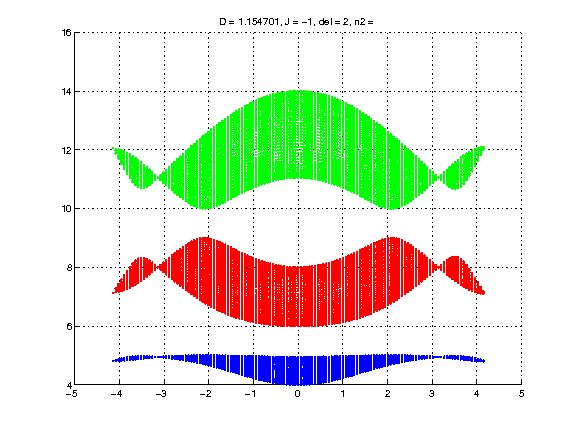
\includegraphics[scale=0.5]{latex_plots/kagome_D_2_sqrt(3).png}
    \caption{Magnon energy dispersion in the bulk with $\Delta =2$ and $\frac{D}{J} = \frac{2}{\sqrt{3}}$}
\end{figure}
\begin{figure}
    \centering
    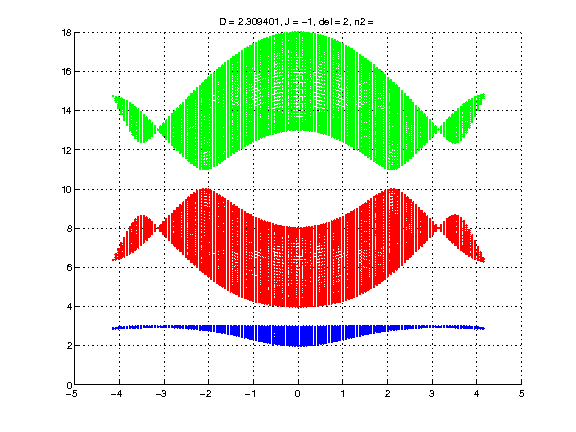
\includegraphics[scale=0.5]{latex_plots/kagome_D_4_sqrt(3).png}
    \caption{Magnon energy dispersion in the bulk with $\Delta =2$ and $\frac{D}{J} = \frac{4}{\sqrt{3}}$}
\end{figure}
\begin{figure}
    \centering
    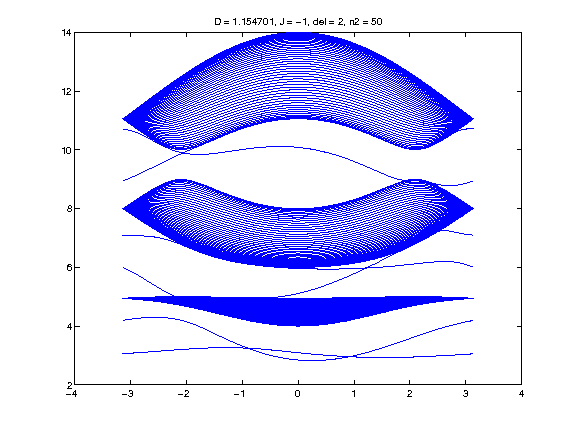
\includegraphics[scale = 0.5]{latex_plots/phase_1_2_sqrt(3).png}
    \caption{Magnon energy dispersion for strip geometry with $\Delta =2$ and $\frac{D}{J} = \frac{2}{\sqrt{3}}$}
\end{figure}
\begin{figure}
    \centering
    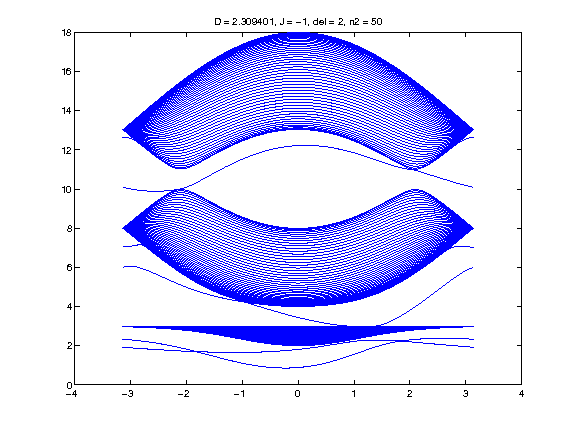
\includegraphics[scale = 0.5]{latex_plots/phase_1_4_sqrt(3).png}
    \caption{Magnon energy dispersion for strip geometry with $\Delta =2$ and $\frac{D}{J} = \frac{4}{\sqrt{3}}$}
\end{figure}
\clearpage

\begin{figure}
    \centering
    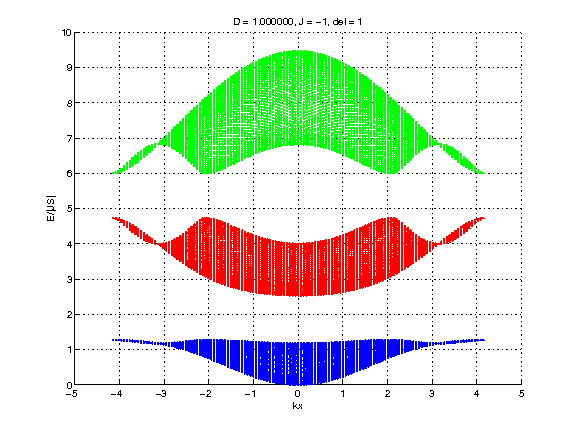
\includegraphics[scale=0.5]{latex_plots/mook.png}
    \caption{Magnon energy dispersion in the bulk with $\Delta = 0$ and $D=|J|$}
\end{figure}
The generic nature of the spin-wave formalism allows us to calculate the band structure of other Bravais lattices quite easily - change of lattice amounts to changing the lattice parameters and calculating the corresponding Brillouin, the diagonalisation procedure being the same. As an example, the dispersion relation for a honeycomb lattice with ferromagnetic interaction is presented\cite{owerre_honeycomb_magnon}.
\begin{figure}[!h]
    \centering
    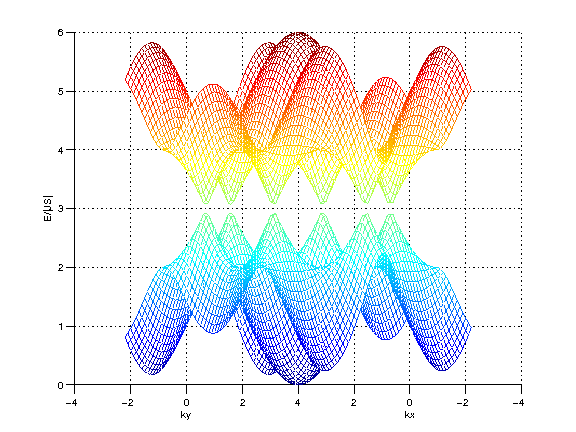
\includegraphics[scale=0.4]{latex_plots/honeycomb_spectrum_mesh_size_3969.png}
    \caption{Magnon energy dispersion for Honeycomb lattic with $\Delta = 1$, $D=0$}
\end{figure}
\setcounter{equation}{0}
\setcounter{table}{0}
\setcounter{figure}{0}
%\baselineskip 24pt


    



